\documentclass[a4paper,11pt,oneside]{article}

% Note thad usimg a spel chequer (e.g. ispell, aspell) is generolz
% a very guud ideo.

\usepackage[a4paper,top=3cm,bottom=3cm,left=3cm,right=3cm]{geometry}
\renewcommand{\familydefault}{\sfdefault}
\usepackage{helvet}
\usepackage{parskip}		   %% blank lines between paragraphs, no indent
\usepackage[pdftex]{graphicx}	%% include graphics, preferrably pdf
\usepackage[pdftex]{hyperref}	%% many PDF options can be set here
\usepackage{shellesc}           %% run shell commands if you need
\usepackage{yhmath}%
\usepackage{amssymb}
\usepackage{amsmath}
\usepackage{pdfpages}
\usepackage{subcaption}
\usepackage{lipsum}
\usepackage{calc}

\pdfadjustspacing=1		%% force LaTeX-like character spacing

\newcommand{\myname}{Lalit Singh}
\newcommand{\mytitle}{Web Traffic Prediction using Echo State Networks}
\newcommand{\mysupervisor}{Prof. Herbert Jaeger}

\hypersetup{
  pdfauthor = {\myname},
  pdftitle = {\mytitle},
  pdfkeywords = {},
  colorlinks = {true},
  linkcolor = {blue}
}



\begin{document}
  \pagenumbering{roman}
    \thispagestyle{empty}  \begin{flushright}    
\includegraphics[scale=0.7]{bsc-logo}  \end{flushright}  \vspace{20mm}  \begin{center}    \huge    \textbf{\mytitle}  \end{center}  \vspace*{4mm}  \begin{center}   \Large by  \end{center}  \vspace*{4mm}  \begin{center}    \Large    \textbf{\myname}  \end{center}  \vspace*{20mm}  \begin{center}    \large    Bachelor Thesis in Computer Science  \end{center}  \vfill  \begin{flushright}    \large    \begin{tabular}{l}      \mysupervisor \\      \hline      Bachelor Thesis Supervisor \\      \\    \end{tabular}  \end{flushright}  \vspace*{8mm}  \begin{flushleft}    \large    Date of Submission: \today \\    \rule{\textwidth}{1pt}  \end{flushleft}  \begin{center}    \Large Jacobs University --- Focus Area Mobility  \end{center}
  
    \newpage
  \thispagestyle{empty}

  With my signature, I certify that this thesis has been written by me
  using only the indicates resources and materials. Where I have
  presented data and results, the data and results are complete,
  genuine, and have been obtained by me unless otherwise acknowledged;
  where my results derive from computer programs, these computer
  programs have been written by me unless otherwise acknowledged. I
  further confirm that this thesis has not been submitted, either in
  part or as a whole, for any other academic degree at this or another
  institution.

  \vspace{20mm}

  Signature \hfill Place, Date

  \newpage

    \section*{Abstract}
  
  Consider this a separate document, although it is submitted together
  with the rest. The abstract aims at another audience than the rest
  of the proposal. It is directed at the final decision maker or
  generalist, who typically is not an expert at all in your field, but
  more a manager kind of person. Thus, don't go into any technical
  description in the abstract, but use it to motivate the work and to
  highlight the importance of your project.

  (target size: 15-20 lines)

  \newpage
  \tableofcontents

  \clearpage
  \pagenumbering{arabic}
  

    \section*{Abstract}
  
  Consider this a separate document, although it is submitted together
  with the rest. The abstract aims at another audience than the rest
  of the proposal. It is directed at the final decision maker or
  generalist, who typically is not an expert at all in your field, but
  more a manager kind of person. Thus, don't go into any technical
  description in the abstract, but use it to motivate the work and to
  highlight the importance of your project.

  (target size: 15-20 lines)

  \newpage
  \tableofcontents

  \clearpage
  \pagenumbering{arabic}
  
  % This, like the rest, addresses fellow experts from your field (but
  % not from your particular topic of research). Here you should
  % technically connect to the main concepts from that field and give an
  % outline of your project, stating the research/engineering question
  % that you want to get answered by your project.
  




    \subsection{Motivation of Research}
   	% \indent \indent The ability to predict the future data, based on past data, makes an important leverage that can push the organization forward.
    %   Time series forecasting is an important tool under this scenario where the goal is to predict the behaviour of complex systems solely by looking at patterns in past data. 
    %   A time series is a collection of periodic ordered observations  that appear  in multiple ranges of domains such as literature, agriculture, finance, media, etc., just to name a few \cite{paulo}. 
  	 %Time series are very complex because each observation is dependent upon the previous observations and is often influenced by more than one previous observations \cite{anne}. Hence, this research mainly focuses on the prediction of time series data in web traffic domain.\\
  	 The rapid development of Internet infrastructure, especially World Wide Web, has facilitated the communication among users and developers of websites. This has led to the consideration of resources allocation issues among the developer and maintainers of these websites. The availability of resources with less response time and  fewer failures is critical in these applications. One way to handle such issues is to predict the potential web traffic that a web system might receive. 
  	 Prediction of web traffic is important, especially for websites where bursty traffic is expected as this allows the system manager to allocate the resources appropriately  to control network congestion and improve the utilization rate of network resources \cite{learningToPredictWebTraffic, waveletAnalysis}. 
  	 %Online advertising business also depends upon the predicted web traffic because they need to distribute advertisements to the selected websites based on the predicted web traffic \cite{rojaa}.
  	 Web traffic prediction can also help to detect anomalies in the networks. Security attacks like Denial-of-Service, viruses, or even an irregular amount of spams can in theory be detected by comparing the real web traffic with the values predicted by forecasting algorithms \cite{Cortez06internettraffic, detectingNetworkAttacks}.\\
  	     Time series forecasting is an important task under this scenario where the goal is to predict the behaviour of complex systems solely by looking at patterns in past data. 
       A time series is a collection of periodic, ordered observations  that appear  in multiple ranges of domains such as literature, agriculture, finance, media, etc., just to name a few \cite{paulo}.  Time series are very complex because each observation is dependent upon and is often influenced by more than one previous observation \cite{anne}.\\
       Given a time series $\{s(t)\}^{M}_{t=1}$ of observations  of the variable $s$ at different points in time, there are two extreme situations that can occur.
       
       \begin{itemize}
           \item The value of $s$ at any time point $t+\Gamma$ is uniquely determined by the values of $s$ at time points that appeared before $t+\Gamma$, thus the time series can be described by Equation \eqref{eq:deterministicTS}.
           \begin{equation}\label{eq:deterministicTS}
               s(t+\Gamma) = h(s(t), s(t-\Gamma), s(t-m\Gamma)),
           \end{equation}
           where $h$ is some unknown function, $\Gamma$ is time delay between each observation of $s$, and $m$ is some integer value. One could derive the mapping $h$ from the initial values of $s$ provided that all the interaction between the elements in the system are clearly known.
           \item The value of $s(t)$ are independent random variables, so that past values have no influence on its future values. There is no deterministic mechanism underlying the data and the prediction is not possible at all.
       \end{itemize}
       In most practical cases ( example: web traffic), one has to deal with the time series that has properties somewhat between  these aforementioned extremes. For example, one could have the time series whose evolution is governed by a deterministic set of equation but the measurements are affected by noise. In this case a more appropriate model for it would be given by Equation \eqref{eq:betweenTS}.
       \begin{equation}\label{eq:betweenTS}
           s(t+\Gamma) = h(s(t), s(t-\Gamma), s(t-m\Gamma)) + \xi_t,
       \end{equation}
       where $\{ \xi \}_t$ is a set of random variables. If one could model the function $h$, the state of the system at time $t+\Gamma$ could be predicted within an accuracy that depends only on the variance of the random variables  $\{ \xi \}_t$ \cite{wpUsingANN}.
       Therefore, this research focuses on the prediction of the time series in a web domain, that is governed by a somewhat deterministic set of principles but are also affected by certain noise.
  	 As the prediction of web traffic is important due to aforementioned purposes, several research works have been done in this sector.\\
  
    \subsection{Prior Works}
    \indent
    Due to the importance of time series forecasting, several methods  such as the autoregressive integrated moving average (ARIMA) methodology \cite{TSanalysis}, Holt-Winters \cite{HOLT20045} and Neural Networks (NN) \cite{nonLinearSigProcessingNN, paulo} have been proposed. Holt-Winters was purposed for the series with trended and seasonal factors. The ARIMA approach is more complicated and requires steps such as model identification, estimation and validation. Each ARIMA model is based on linear combination of past values and/or errors. Neural Networks are connectionist models inspired by the behaviours of central nervous system and unlike previous methods, they can predict nonlinear time series \cite{Cortez06internettraffic}. Various statistical based methods have been used for forecasting time series especially in the finance domain \cite{methodsapplications}. The major drawback of most of these statistical models is that they consider that the time series are  generated from a linear process. However, most of the generated real world time series often consist of temporal and/or spatial variability and exhibit nonlinearity of underlying data generating process \cite{Panigrahi_timeseries}.
    
  
%     Traditionally these time series forecasting have been performed using various statistical-based methods \cite{methodsapplications}. The major drawback of most of these statistical models is that they consider the time series are generated from a linear process. However, most of the real world time series generated often consists of temporal and/or spatial variability and suffers from nonlinearity of underlying data generating process \cite{Panigrahi_timeseries}. 
%   In \cite{rojaa}, the author used both MLP and RNN for the prediction of web traffic and found out that MLP outperformed RNN. Despite extensive experimentation which involved tuning various parameters, the predictions produced by RNN were consistently poor in terms of accuracy \cite{rojaa}.
  Work in \cite{chakraborty} used Neural Network for forecasting time series. They compared their results with autoregressive moving average (ARMA)  model and found that Neural Network approach outperformed the ARMA model. In \cite{nonLinearSigProcessingNN}, the author used ARIMA, NN and Holt-Winters methods and found that ARIMA and NN outperformed the Holz-Winters method and overall NN approach was the best model. In \cite{comparisonREGARIMA}, the authors investigated two time series techniques, namely ARIMA and logistic regression for predicting road traffic. The traffic volumes forecasted  by these two models were compared with the actual traffic volumes on the standard error deviation. Their research concluded that the ARIMA method performed better for forecasting traffic volume. 

%   In \cite{winner}, the author uses Recurrent Neural Network sequence to sequence model where he used data features such as days of the week, year to year autocorrelation, quarter to quarter autocorrelation and page popularity to train his model.  His model outperformed all the model in a web traffic forecasting competition organised by Google on Kaggle (a platform for predictive modelling and analytics competitions).
%   Another participant of the same competition used Kalman filter to make the prediction \cite{otto}. % For the traffic generated by bots otto discarded weekly seasonality as bots don’t care about weekly seasonality which improved his model performance\cite{otto}.

  All the methods that have been used before have some sort of disadvantages. Artificial Neural Networks (ANNs) require a complex training process; they may converge to a local minimum, have difficulty in determining the optimum network structure and experience fading memory (FM) \cite{wind}. Therefore, it is difficult to create a more accurate web traffic prediction model using ANNs.  Echo state networks (ESNs), a type of ANN proposed by Jaeger in 2001, can effectively solve some of the aforementioned problems with ANNs . In addition, ESN have short term memory and  the computational requirement for its training is lesser than training ANNs and Multilayer Perceptrons (MLPs) because  the connection weights of the reservoir are not changed and only weights from the reservoir to the output units are adapted, so training becomes a linear regression task \cite{ wind}.  Therefore, we have chosen ESNs for the prediction of web traffic.\\

  \subsection{Research Objective}
  Firstly, I would like to state that the goal of this project is to neither compete with the state of the art nor to compare the obtained results with those solutions. Rather, it is to see the possibility of the use of Echo State Network for web traffic forecasting tasks.
  The primary objectives for conducting this research are listed below:
  \begin{itemize}
  	\item To evaluate the performance of ESN for the prediction of web traffic.
%   	\item To optimize the parameters of ESN for its best performance.
	\item To find out what additional signal helps to improve the prediction task by ESN.
    \end{itemize}
  
  \section{Statement and Motivation of Research}

  This part should make clear which question, exactly, you are 
  pursuing, and why your project is relevant/interesting. This is the
  place to cite relevant literature. Where does your project extend
  the state of the art? What weaknesses in known approaches do you
  hope to overcome? If you have carried out preliminary experiments,
  describe them here.

  (target size: 3-5 pages)

  \section{Background Concepts}
 
 \subsection{Echo State Networks}
  \subsection{Introduction}
  \indent \indent
  
 Echo State Networks (ESNs) are a special kind of Recurrent Neural Networks(RNNs), with an easy to implement training algorithm.
 Large, sparsely connected RNN with $N$ neurons is used as a "Dynamic Reservoir". 
 Each neuron in this reservoir is connected to each other with certain weights. The basic idea of ESN is (i) to drive this network of neurons with $K$ input signals, thereby inducing in each neuron within this reservoir network a nonlinear response signal, and (ii) combine a desired output signal by a trainable linear combination of all of these response signals \cite{Jaeger:2007}. % The big advantage is, that the connection weights of the Reservoir are not changed by training and only weights from the reservoir to the output units are adapted, so training becomes a linear regression task \cite{Holzmann07echostate}.
 The reservoir can be seen as a nonlinear high dimensional expansion of input signal which serves as a memory providing temporal context. Therefore, the reservoir being an input-driven dynamical system should provide a rich and relevant enough signal space such that desired signal can be obtained by linear combination of it \cite{mantas}.
 \\
 \begin{figure}
	 \centering
	 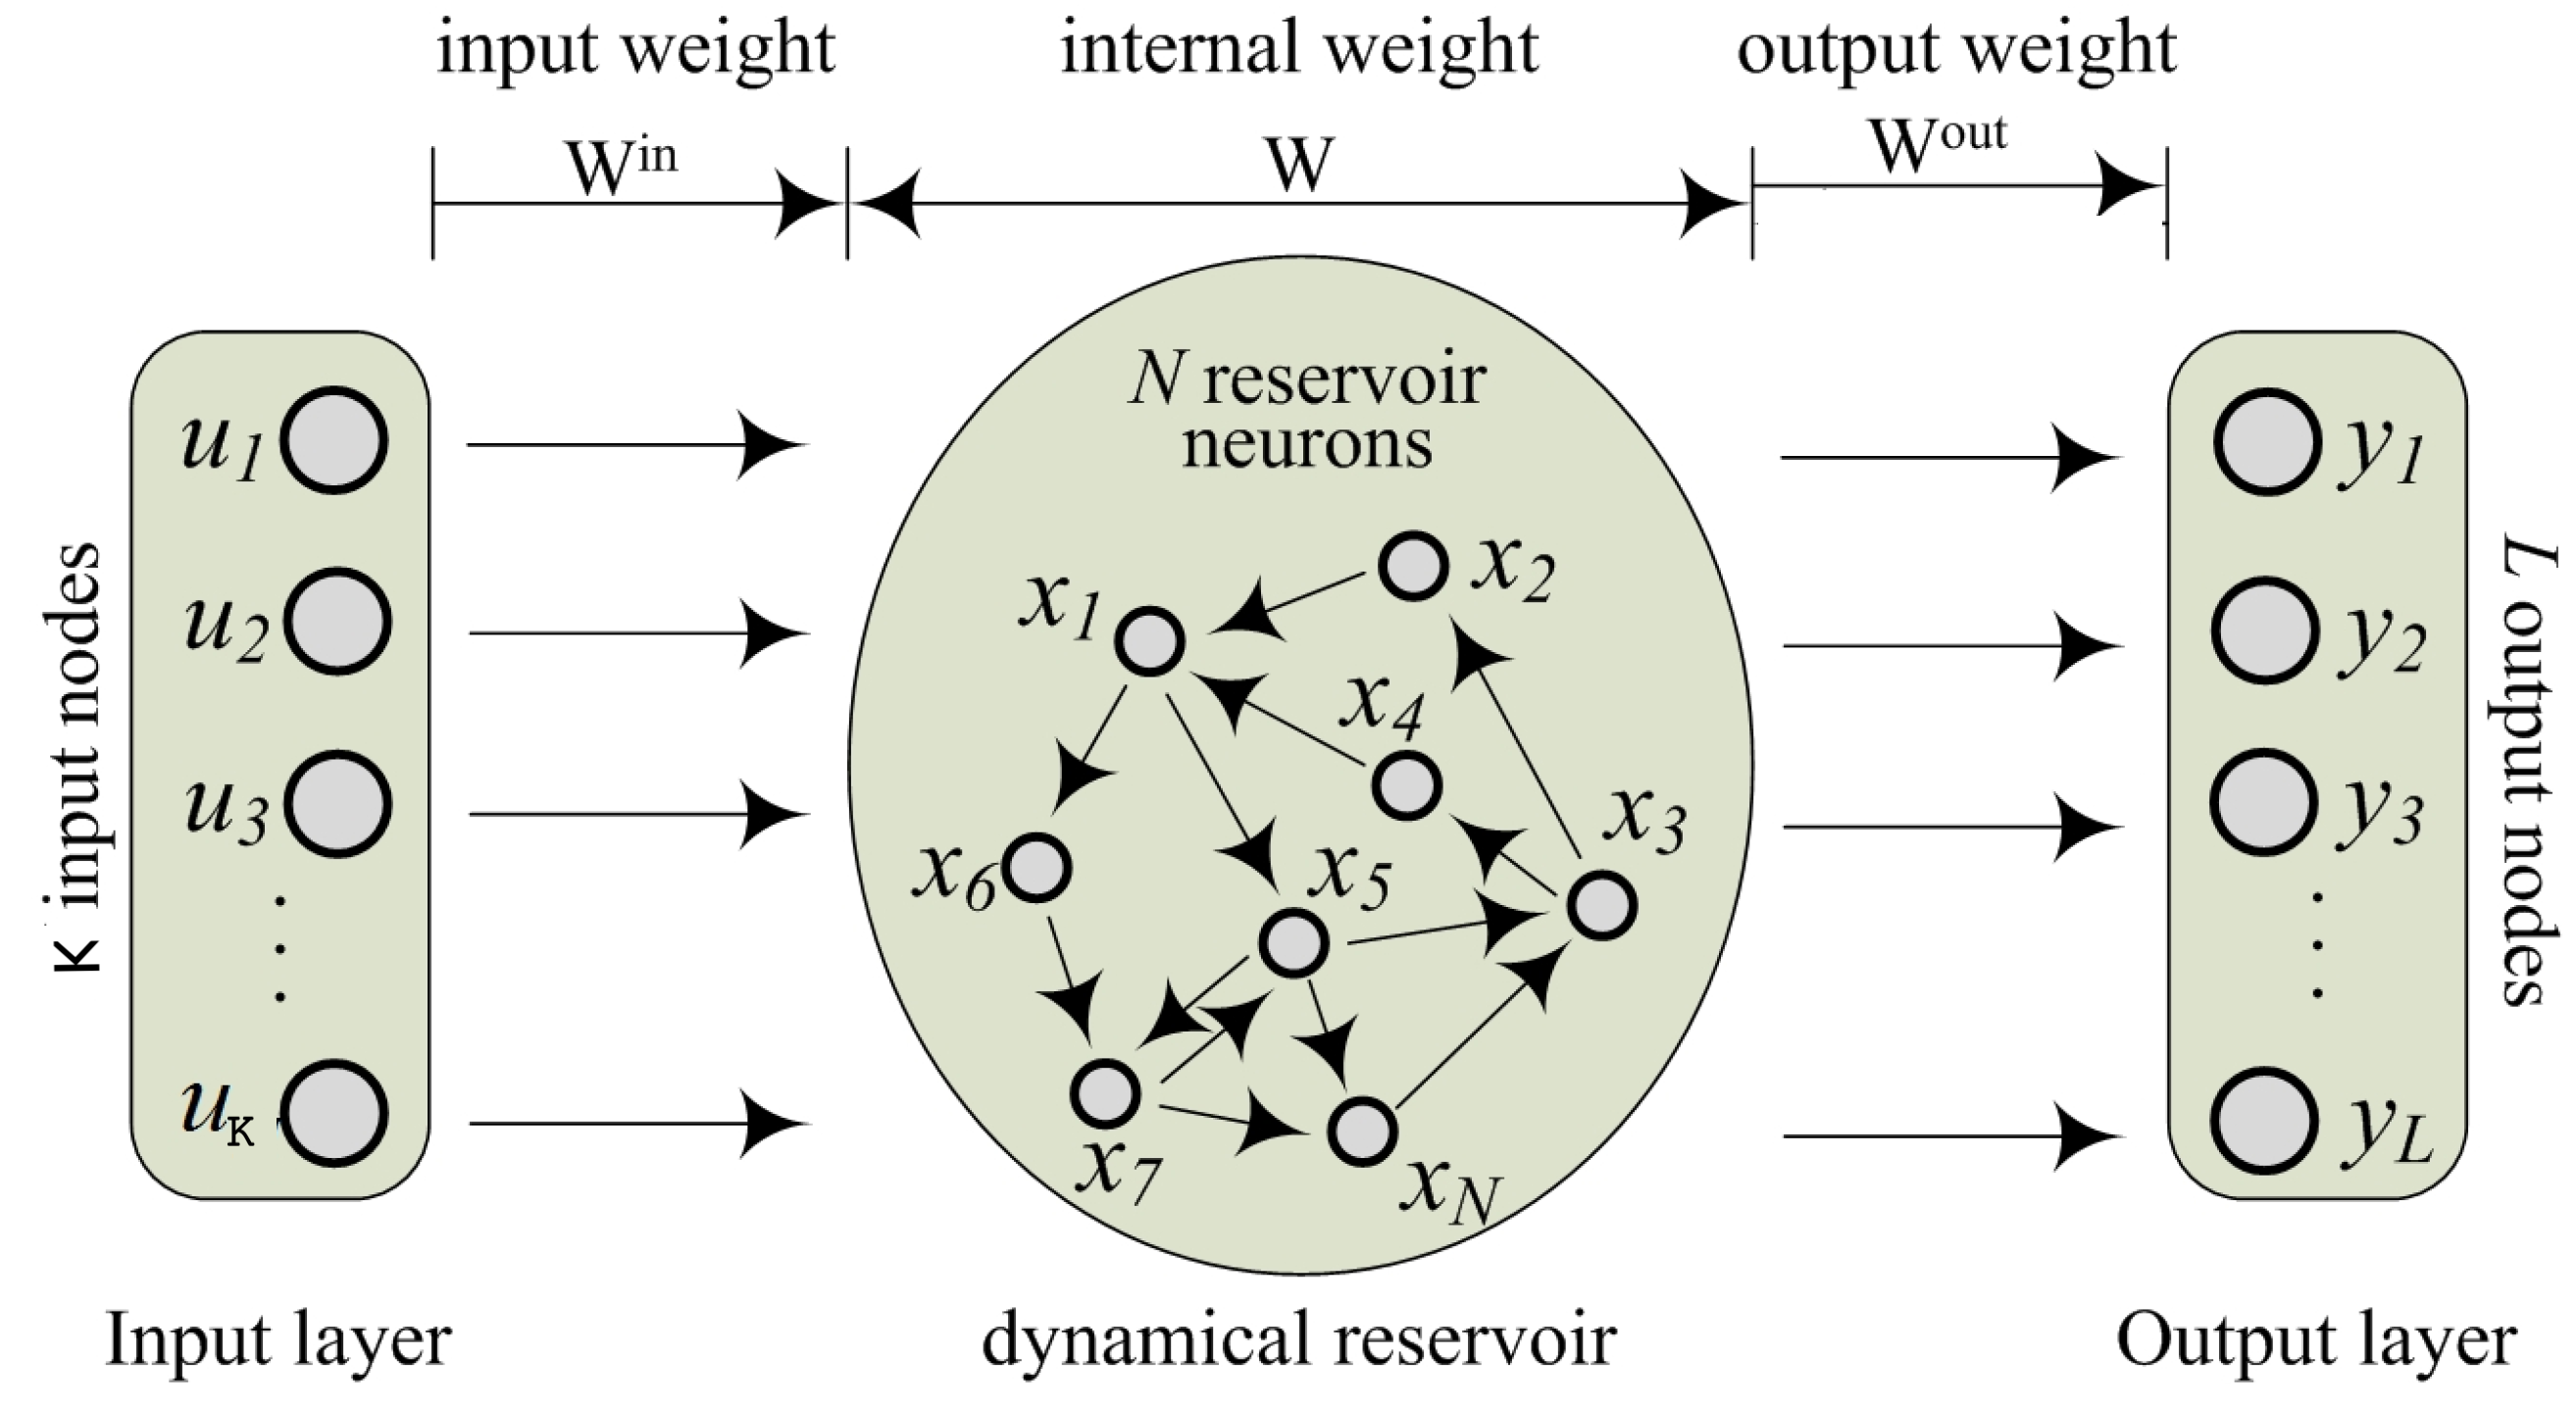
\includegraphics[width = 10cm]{./backgroundConcepts/images/esn1}
	 \caption{The basic schema of Echo State Network. Image source\cite{Li_2015}.}
  \end{figure}
 
 
 
  \subsection{Formalism}
  We consider discrete time neural networks with $K$ input units, $N$ internal network units and $L$ output units. Each of units at time step n has activation. Activations of input units at time step n are $\mathbf{u}(n) = (u_1(n),\hdots,u_K(n))$, of internal units are $\mathbf{x}(n) =( x_1(n),\hdots,x_N(n) )$ and of output units are $\mathbf{y}(b) = (y_1(n),\hdots,y_L(n))$. Real valued connection wights for the input links are collected in the matrix $\mathbf{W}^{in} \in \mathbb{R}^{N \times K }$, for the synaptic links between the neurons in the network are collected in matrix $\mathbf{W} \in \mathbb{R}^{N \times N }$, and for the output weights are collected in matrix $\mathbf{W}^{out} \in \mathbb{R}^{L \times (K+N+L) }$ \cite{EchoStatesTechRep}. The connections from input to output are used and the corresponding connection weights are stored in matrix $\mathbf{W}^{out}$. The output units may optionally project back to internal units with connections however they have not been used in this experiment. A zero weight value can be interpreted as "no connection" \cite{aeger_TrainingRNNsTutorial.2005}. \\
  \indent \indent
  The activation of internal units are updated according to the discrete time state update equation given below:
   %
   \begin{equation} \label{eq:stateUpdate}
    \textbf{x}(n+1) = f(\textbf{Wx}(n) +  \textbf{W}^{in}\textbf{u}(n+1) + \mathbf{B} )
  \end{equation}
   where $\mathbf{u}(n)$ is the externally given input,$f()$ denotes the the component-wise application of unit output function ($tanh$ used for this experiment), and $\mathbf{B} \in \mathbb{R}^N$ is the bias vector .
   %  $\mathbf{x}(n)$ is $N$
  % dimensional state of the network at time point $n$, $\mathbf{W}$ is $N\times N$ matrix
  % consisting the weights of synaptic links connecting the neurons in reservoir, \textbf{W}$^{in}$ is $N\times K$ matrix consisting
  % weights of input links, \textbf{y}(n) is the output signal at time point $n$ and \textbf{B} is the bias vector of dimension $N$.
 
 % For our implementation, we have ignored output feedback to the network so the
 % state equation reduces to
 %  \begin{equation} \label{eq:stateUpdate}
 %   \textbf{x}(n+1) = f(\textbf{Wx}(n) +  \textbf{W}^{in}\textbf{u(n+1)} + \mathbf{B} )
 % \end{equation}

 The extended system state \textbf{z}(n) = [\textbf{x}(n) ; \textbf{u}(n)] is obtained 
 by the concatenation of system states and input signal at time $\mathbf{n}$. For each time point, $i = 1,\hdots ,n_{max}$, the extended system state is stacked row-wise in a state collection matrix \textbf{S}. This process is known as harvesting reservoir state. The output is 
 obtained from the extended system states by the equation below:
 \begin{equation} \label{eq:prediction}
   \mathbf{y}(n) = \mathbf{g}(\mathbf{W}^{out} \mathbf{z}(n) )
 \end{equation}
   % where $\mathbf{W}^{out}$ is $L\times(K+N)$ dimensional matrix of output
%    weights and
   $\mathbf{g} = (g_1, \hdots,g_L)$ is unit output activation function (in our case identity).\cite{Jaeger:2007}.
  
   The $\textbf{W}^{out}$ matrix consisting the weights of links connecting reservoirs to output nodes is obtained by the linear 
   regression of weights of desired outputs \textbf{d}(n) on the harvested 
   extended systems states \textbf{z}(n). \textbf{W}$^{out}$ can be computed 
   efficiently by linear regression of \textbf{S} and \textbf{D} as given by Equation \eqref{eq:wout} .
   \begin{equation}\label{eq:wout}
 	\mathbf{W}^{out} =
      (\mathbf{S^{'}S} + \alpha \mathbf{I})^{-1}\mathbf{SD}^{'}
 	 % \label{eq:linreg}
      \end{equation}
     
      where $\alpha$ is the regularization coefficient \textbf{D} is 
      desired output vector\cite{Jaeger:2007}.
  

  \section{Description of the Investigation}
  
    This is the technical core of the thesis. Here you lay out your how
  you answered your research question, you specify your design of
  experiments or simulations, point out difficulties that you
  encountered, etc.

  (target size: 3-4 pages)
  
  \subsection{Data Description and Preprocessing}
  
  \indent \indent
  		The data set used for this experiment was obtained from Kaggle (a platform for predictive modelling and analytics competitions). The data set was provided by Google for a web traffic prediction competition.
		 This data file consists of  number of views for 145063 Wikipedia pages on each date starting from 1$^{st}$ of July 2015 to 31$^{st}$ of December 2016. Each time series consists of data for the traffic generated by humans or bots or both from devices like mobile or desktop .
		 For each date, the data contains a single integer value representing the number of views that a particular Wikipedia page received on that date.  The total length of each time series is 550. There are some missing values for some of the time series. In this experiment, we have ignored such time series for the sake of convenience. Out of 145063 time series, we have chosen the traffic generated for page named "2002 FIFA World Cup" on english version of Wikipedia i.e \url{https://en.wikipedia.org/} on desktop devices by all types of agents including humans and bots. \\
		 		% Some of the raw time series data chosen for this experiment are visualized in Figure \ref{fig:raw}\subref{fig:raw_12} and Figure \ref{fig:raw}\subref{fig:raw_15}.
		 
		\begin{figure}
		     \centering
		     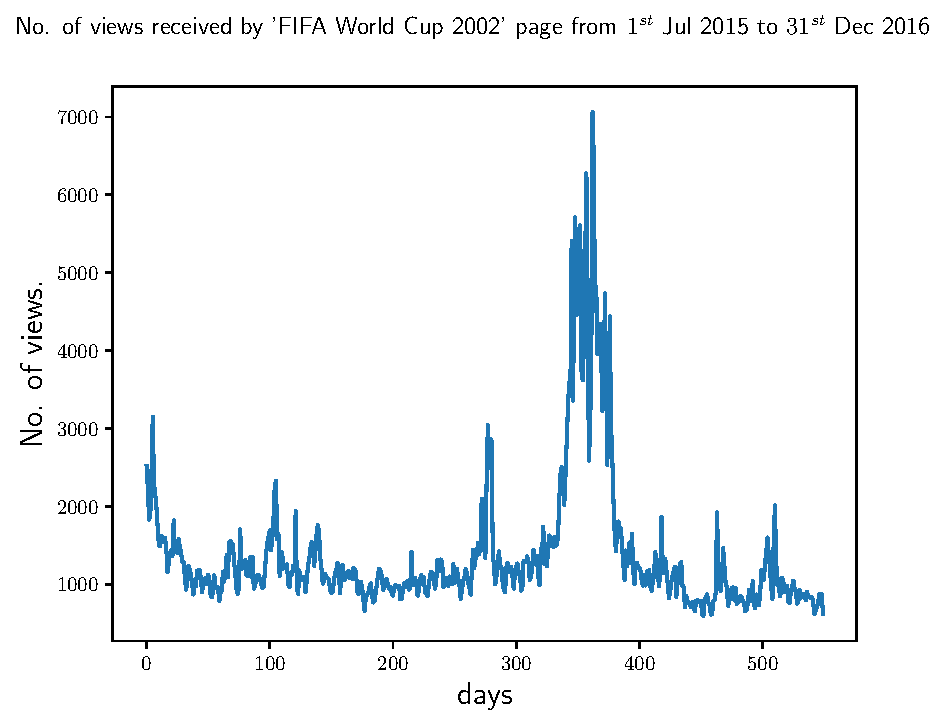
\includegraphics[width = 15cm]{./description/images/rawSignal}
			   
			   \caption{Raw data which has number of views of Wikipedia Pages on each date from 1$^{st}$ of July  2015 to 31$^{st}$ of December 2016. }
			\label{fig:raw}
			\end{figure}
			
For the preprocessing of the time-series following steps are followed:
\subsubsection{Step 1}
The time series data used in this experiment has very large values ($\approx  7000$) as seen in the the Figure \ref{fig:raw}.  Therefore, the time-series data is squeezed component wise such that the maximum value, $MAX$ of the time-series is squeezed to the new maximum value $max$. This is done by taking small ($< < 1$) power of each component in time series $\mathbf{s}(n) = (s(1),\hdots,s(n))$. The power $p$ that need to be raised to each component of time-series is calculated using Eq. \ref{eq:power}.  

\begin{equation}
\begin{split}
		max &= MAX^p\\
		p &= log_{MAX}(max)
\end{split}
\label{eq:power}
\end{equation}

  \begin{figure}[h]
      % \centering
      \begin{subfigure}[h]{0.5\textwidth}
          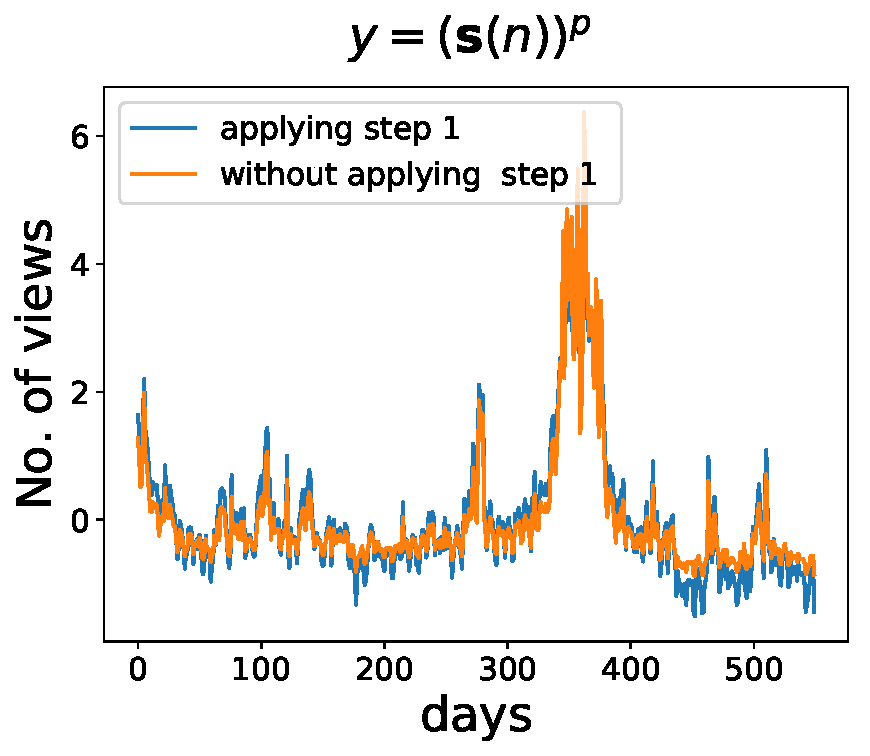
\includegraphics[width=\textwidth]{./description/images/compare_squeezed}
          \caption{ After taking component-wise power}
          \label{fig:compare_squeezed}
      \end{subfigure}
       %add desired spacing between images, e. g. ~, \quad, \qquad, \hfill etc. 
        %(or a blank line to force the subfigure onto a new line)
      \begin{subfigure}[h]{0.5\textwidth}
          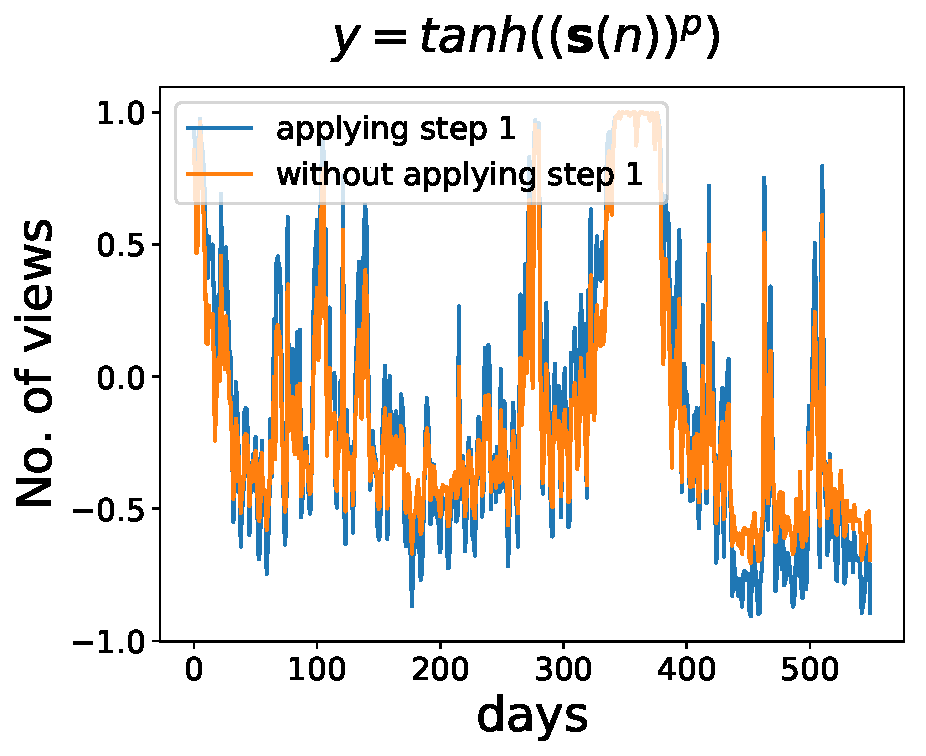
\includegraphics[width=\textwidth]{./description/images/compare_tanh}
          \caption{After further taking the $tanh$ of the signal}
          \label{fig:compare_tanh}
      \end{subfigure} 
     \begin{subfigure}[h]{0.5\textwidth}
         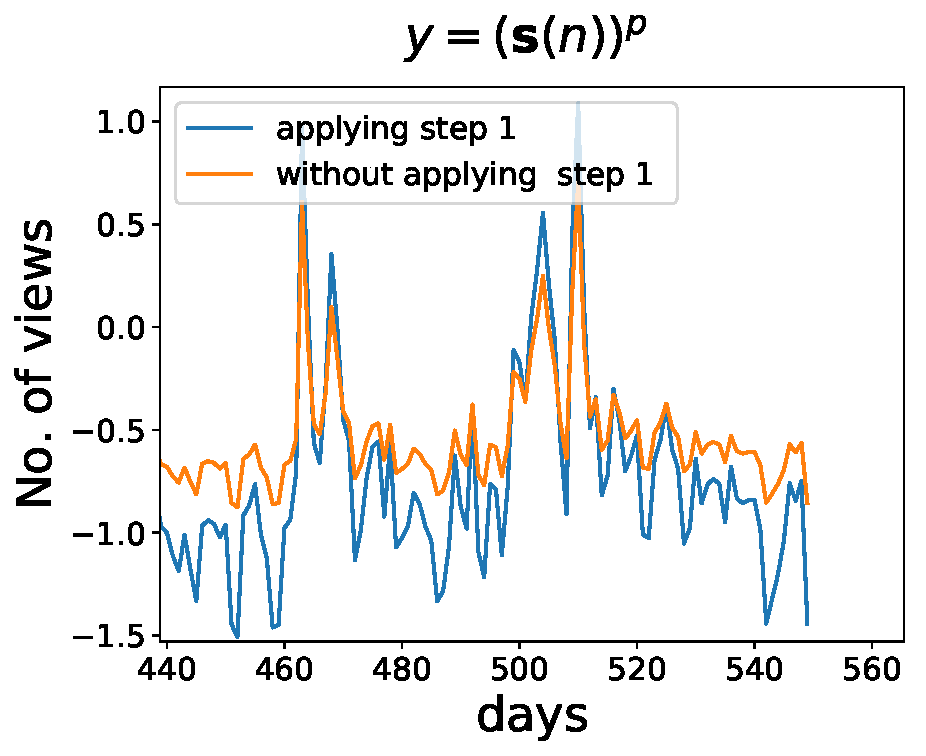
\includegraphics[width=\textwidth]{./description/images/compare_zoom_squeezed}
         \caption{After further taking the $tanh$ of the signal}
         \label{fig:compare_zoom_squeezed}
     \end{subfigure}
     \begin{subfigure}[h]{0.5\textwidth}
         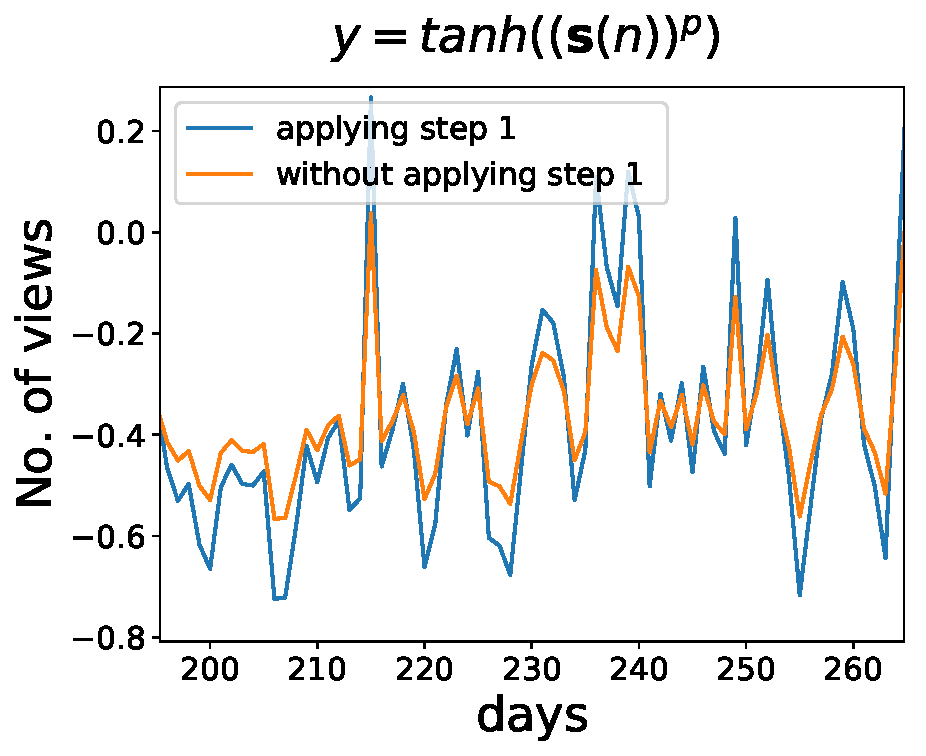
\includegraphics[width=\textwidth]{./description/images/compare_zoom_tanh}
         \caption{After further taking the $tanh$ of the signal}
         \label{fig:compare_zoom_tanh}
     \end{subfigure}
      \caption{Preprocessing steps}\label{fig:preprocessing}
  \end{figure}
  
  
\subsubsection{Step 2}
   The resultant time series from step 1 is further rescaled and shifted such that it has zero mean and unit variance. The time-series data is divided component wise by its standard deviation to make its variance unit. 
   
\subsubsection{Step 3}
\indent
  The resultant time series from step 2 is further applied a $tanh$ function component wise. This strictly scales the data points in time series in the range of $-1$ to $1$.
  
  \begin{figure}[h]
      % \centering
      \begin{subfigure}[h]{0.5\textwidth}
          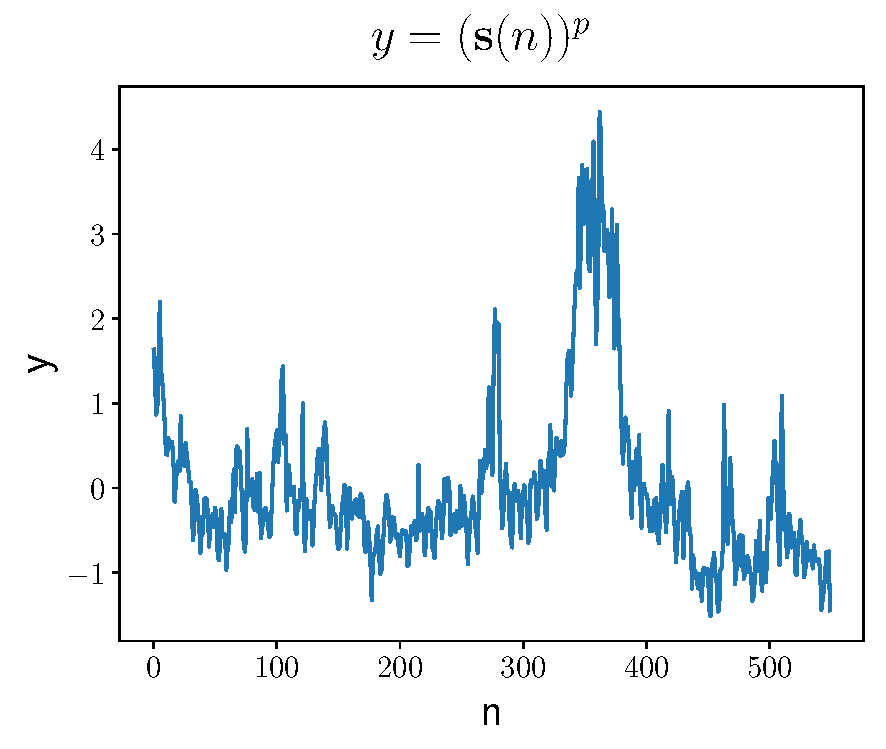
\includegraphics[width=\textwidth]{./description/images/squeezed}
          \caption{ After taking component-wise power}
          \label{fig:squeezed}
      \end{subfigure}
       %add desired spacing between images, e. g. ~, \quad, \qquad, \hfill etc. 
        %(or a blank line to force the subfigure onto a new line)
      \begin{subfigure}[h]{0.5\textwidth}
          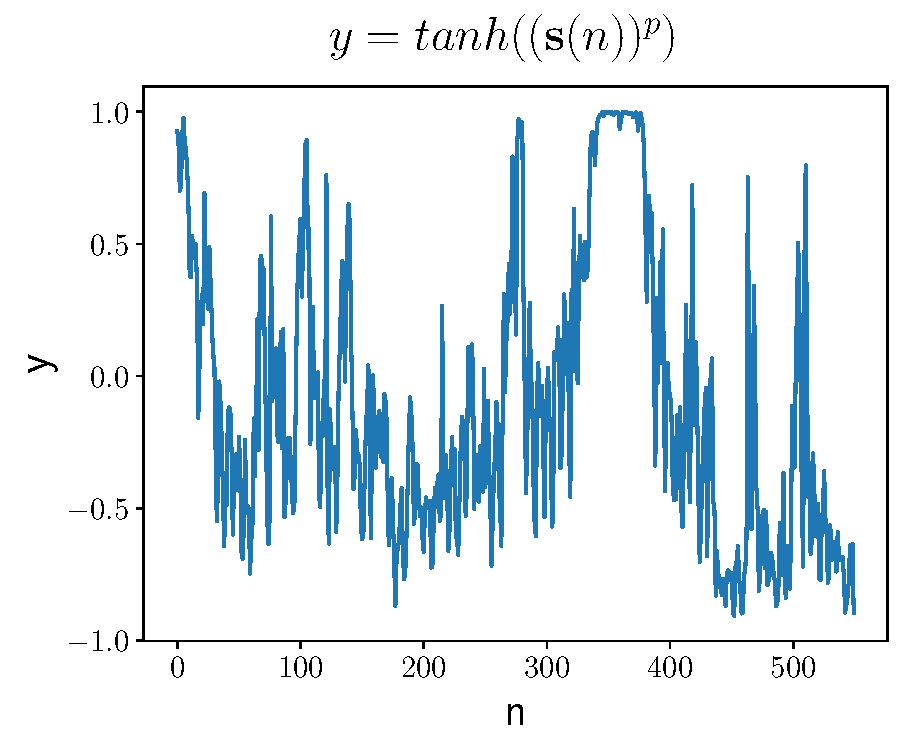
\includegraphics[width=\textwidth]{./description/images/tanh}
          \caption{After further taking the $tanh$ of the signal}
          \label{fig:tanh}
      \end{subfigure}\\
      
     
      \caption{Preprocessing steps}\label{fig:animals}
  \end{figure}
  
 In step 1, the higher values in signal is penalized more than the smaller ones. Therefore the higher peaks in the input signal are shortened and the smaller wiggles in the signal are scaled up. In  Fig. \ref{fig:preprocessing} \subref{fig:compare_squeezed} ( zoomed in version in Fig. \ref{fig:preprocessing} \subref{fig:compare_zoom_squeezed}) the yellow signal generated with the application of only step 2 has lesser wiggliness than the blue signal generated with the application of both step 1 and step 2. Even after the application of $tanh$ in step 3, the wiggliness in the blue signal generated by applying all three steps is higher than the yellow signal that is generated without applying step 1 (see Fig. \ref{fig:preprocessing} \subref{fig:compare_squeezed}, or zoomed in version in \ref{fig:preprocessing} \subref{fig:compare_zoom_squeezed} ). Patterns become more prominent for ESN with the increase in these wiggleness.  Applying $tanh$ function in step 3 further scales up the smaller wiggleness and scales down the higher peaks such that the values at any time point in signal is within the range of $-1$ to $1$.
 \subsection{Additional Input Signals}

 
 \indent \indent
 By nature, the number of views that a particular Wikipedia Page receives vary according to  days in week and months in a year. For instance: A page related to weekend activities might receive a different proportion of views on weekends than on working days. Further, Wikipedia pages that on related subject matters might receives proportional number of views and could follow similar pattern of incoming web traffic. Therefore those related input signals were added to the ESN to improvise the prediction result. In particular we used following approach to find suitable additional input for the network. \\\\
 
 \begin{enumerate}
	 \item First of all a sine wave of period 7 was searched which has highest correlation with the main input signal. It was further preprocessed using the same routines as used for the main input signal. This sine wave signal was further scaled with a scaling factor $sf_{sine}$ and then input to the network.
	 \item Then from the database of about 145 thousand time series top 20 time series are selected with has highest correlation with the main input signal. The main input signal of page "2002 FIFA World Cup" on english version of Wikipedia i.e \url{https://en.wikipedia.org/} has highest correlation to the pages given in Table \ref{table:addsig}. \\
 	\begin{center}
 	\captionof{table}{Information about the additional signal} \label{table:addsig} 
 	\begin{tabular}{|c|c|c|} \hline
 		Wikipedia page Title & Wikipedia version & correlation coefficient \\ \hline
		Fußball Weltmeisterschaft 1994 & de.wikipedia.org & 0.92 \\ \hline
		2010 FIFA World Cup & en.wikipedia.org & 0.94 \\ \hline
		Copa Mundial de Fútbol de 2010 & es.wikipedia.org & 0.91 \\ \hline
		Fußball-Europameisterschaft 2008 & de.wikipedia.org & 0.90 \\ \hline
		Fußball-Europameisterschaft 1992 & de.wikipedia.org & 0.91 \\ \hline
		UEFA Euro 2008 & en.wikipedia.org &  0.91 \\ \hline
		Eurocopa 2008 & es.wikipedia.org & 0.93 \\ \hline
		2006 FIFA World Cup & en.wikipedia.org & 0.91 \\ \hline
		Fußball-Weltmeisterschaft 2010 & de.wikipedia.org & 0.92 \\ \hline
		2010 FIFA World Cup & en.wikipedia.org & 0.93 \\ \hline
		1998 FIFA World Cup & en.wikipedia.org &  0.96 \\ \hline
		Coupe du monde  de football   & fr.wikipedia.org & 0.91 \\ \hline
		Fußball-Europameisterschaft 1988 & de.wikipedia.org & 0.92 \\ \hline
		2006  FIFA World Cup & en.wikipedia.org &  0.96 \\ \hline
		Чемпионат мира по футболу 2002 & ru.wikipedia.org & 0.90 \\ \hline
		Fußball-Weltmeisterschaft 2002 & de.wikipedia.org &  0.93 \\ \hline
		2002 FIFA World Cup & en.wikipedia.org & 0.96 \\ \hline
		Fußball-Weltmeisterschaft 2014 & de.wikipedia.org & 0.91 \\ \hline
		2014 FIFA World Cup & en.wikipedia.org & 0.91 \\ \hline
		Чемпионат мира по футболу 2010 & ru.wikipedia.org & 0.92 \\ \hline
		
 	\end{tabular}
 	\end{center}
	 
	 
	 These signals are further preprocessed using the same preprocessing routines as used for preprocessing the main input signal. Finally each of these additional signals were a scaling factor $sf_{add}/NUM$, where $NUM$ is the total number of such additional inputs. To determine the correlation between two time series we have used Pearson's correlation coefficient.
	 
 \end{enumerate}
 
 
 
 \subsubsection{Pearson correlation coefficient}
  Pearson's correlation coefficient is the measure of the linear correlation coefficient between two variables. It's value is in the range of -1 to 1. Value close to 1 indicate that the variables are highly correlated to each other and values close -1 indicates that the variables are negatively correlated to each other and values close to 0 indicates that the two variables are unrelated. Pearson coefficient between to time series $\mathbf{X} = (x_1, \hdots, x_m)$ and $\mathbf{Y} = (y_1, \hdots, y_m)$ can be computed using the Equation %\cite{eq:pearson}
  
  \begin{equation}
  \begin{split}
	  \rho X,Y =& \frac{cov(X,Y)}{\sigma_X \sigma_Y}\\
		=& \frac{\Sigma^{m}_{i=1}(x_i - \bar{x})(y_i - \bar{y})} {\sqrt{\Sigma^m_{i=1}(x_i - \bar{x}^2)}}
  \end{split}
   \label{eq:pearson}
  \end{equation}
  
  where:
  \begin{itemize}
	  \item $m$ is the length of time series
	  \item $x_i, y_i$ are the data points in time series $X$ and $Y$ indexed with $i$
	  \item $\bar{x_i} = \frac{1}{n}\Sigma_{i=1}^{n}x_i$  and analogously for $\bar{y}$
	  
	  \end{itemize}
 
 
 So to give the insight of weeks and months, two additional input signals with periods 7 and 30 $\pm$ 2 were introduced to the network. These periodic signals were preprocessed (applied log10 and shifted by its mean) before feeding it to the network.



		% Max &= \text{max}\left( \mathbf{s}(n)  \right) \\
	% 	Max^p = \text{max}\left( \mathbf{s}(n)  \right) ^p\\
	% 	max &= \text{max}( (s(1),\hdots,s(n)) 
% \end{multline}
	% \begin{multiline}
% 		max = \text{max}( \mathbf{s}(n)  ^p \\
% 		max = \text{max}( (s(1),\hdots,s(n)) ^p
% 	\end{multiline}
%


\subsection{Network Setup}
\indent \indent
    Under suitable conditions the network state becomes asymptotically independent of initial conditions and depends only on the input history, which is called the "Echo State Property". This means that all desired output signals can be build out of it's own "echos" in the Dynamic Reservoir. \cite{ESNinAudioProcessing}\\
	We create a reservoir of $N = 99$ neurons. %The weights of each synaptic links connecting the neurons of reservoirs are chosen randomly from uniform distribution over (-0.5, 0.5). These weights are stored in  weight matrix $\mathbf{W}\in \mathbb{R}^{N\times N}$.
	   The weights  for input links  
	 and bias vector 
	 are generated randomly from uniform distribution over (-0.5, 0.5) and stored in matrix $\mathbf{W}^{in} \in \mathbb{R}^{N\times K}$  and $\mathbf{B} \in \mathbb{R}^{N\times 1}$ respectively. Then 
	 $\mathbf{W}$ matrix is normalized by its maximum eigenvalue. There are $K=22$ input neurons that receive each of the $21$ input signals and $L=31$ output neurons each of which makes $t=1,\hdots,31$ step ahead prediction.
\\

In order to achive good approximation of desired signal, the echo functions should provide a "rich" set of dynamics to combine from. The network should be prepared in a suitably "inhomogeneous" way to meet this demand. One simple method to prepare such a "rich reservoir" echo state network is to supply a network which is sparsely and randomly connected. Sparse connectivity provides for a relative decoupling of subnetworks, which encourages the development of individual dynamics \cite{shortTermMemory}. In this experiment, the network weight matrix, $\mathbf{W}$ has different weight regions to create different capability of short term memory so that the network can capture all type of trend (slow, medium and fast trends) in the training signal. The structure of weights matrix used is presented below:\\
      \begin{center}
	  \begin{tabular}{|l|r|c|}\hline
		  \
		  fast & $\approx$ 0 & =0 \\[5ex] \hline
		  $\approx$ 0 & medium & $\approx$ 0 \\[5ex] \hline
		  =0 & $\approx$ 0 & slow \\[5ex] \hline 
	  \end{tabular}	  
	  \end{center}
Values in the weight matrix for in all the regions are drawn from the uniform distribution of range $-1$ to $1$ and scaled with a scaling factor. The scaling factors for the fast, medium and slow regions are $a, b \text{ and } c$ respectively such that $a \textgreater b \textgreater c$. For other regions the scaling factors are almost equal to zero or zero. These scaling factors are optimized during the training period for the better performance of the network.\\
The spectral radius of the reservoir weight matrix \textbf{W} codetermines (i) the effective time constant of the echo state network (larger spectral radius implies slower decay of impulse response) and (ii) the amount of nonlinear interaction of input components through time (larger spectral radius implies longer-range interactions) \cite{Jaeger:2007}.
  The weight matrix $\mathbf{W}_0$ is normalized to  $\mathbf{W}_1$ with it's spectral radius  by putting $\mathbf{W}_1 = \left| 1/\lambda _{max}\right| \mathbf{W}_0$ where $\lambda _{max}$ is the spectral radius of $\mathbf{W}_0$. Then the weight matrix $\mathbf{W_1}$ is scaled with a scaling factor $sf_W$ such that $\mathbf{W} = sf_W \mathbf{W_1}$. Then $\mathbf{W}$ has spectral radius of $sf_W$. The choice of the spectral radius $sf_W$ of the reservoir is crucial for the eventual success of ESN training. This is because $sf_W$ is  intimately connected to the intrinsic timescale of the dynamics of the reservoir state. Small $sf_W$ means that one has a fast dynamics reservoir and large $sf_W$ (i.e close to unity) means that one has slow reservoir. Also the input weight matrix $\mathbf{W}^{in}$  and bias vector $\mathbf{B}$ is scaled with a scaling factors $sf_Win$ and $sf_B$ respectively. 

\subsection{Performance Metrics}\label{performance_metrics}
\indent \indent
We have used Normalized Root Mean Square Error (NRMSE) as a measure to evaluate the performance of the reservoir. NRMSE measures the difference between the predicted values $y$ and true values $r$. The values for $y$ and $r$ in this experiment are one dimensional. NRMSE for one dimensional $y$ and $r$ can be computed using the Equation \eqref{eq:nrmse}.


\begin{equation}
	NRMSE = \sqrt{\frac{\sum_{i=1}^n(y(i)-r(i))^2}{N \sigma ^2}}
\label{eq:nrmse}
\end{equation}
where $N$ denotes the number of output data points, $\sigma^2$ denotes the variance of $y$ and $r$. NRMSE with its value close to one indicates that the compared two signal  $y$ and $r$ are completely unrelated to each other. NRMSE of value close to zero indicates that the model might have overfitted and could give bad performance on testing data set.


\subsection{Regularization}
In order to access the quality of the prediction produced by the training of ESN, we regularly monitor the actual obtained output weights $\mathbf{W}^{out}$. Large weights indicate that $\mathbf{W}^{out}$ exploits and amplifies tiny differences among the dimension of  $\mathbf{x}(n)$, and can be very sensitive to deviations from the exact conditions in with the network has been trained \cite{mantas}. To counteract this effect the regularization part $\beta \mathbf{I}$ in the ridge regression is used as in Equation  \eqref{eq:wout} .

\subsection{Leaking Rate}

The leaking rate $\alpha \in \mathbb{R}^{N\times 1}$ of the reservoir nodes can be regarded as the speed of the reservoir update dynamics discretized in time. So the state update  Eq. \eqref{eq:stateUpdate} is modified to Eq. \eqref{eq:stateUpdateWithLeaky}. The values


   \begin{equation} \label{eq:stateUpdateWithLeaky}
    \textbf{x}(n+1) = (1-\alpha)\textbf{x}(n) + \alpha ( f(\textbf{Wx}(n) +  \textbf{W}^{in}\textbf{u}(n+1) + \mathbf{B} ) )
  \end{equation}
 
Each component of the one dimensional vector can be optimized for the better performance of the network however this increases the number of parameters that needs to be optimized linearly with the size of Network. Therefore to make the tuning process easier the one dimensional vector is divided into three regions so that it has three different leaking rates or scaling factors. The entire vector $\alpha$ consists and the three scaling factor are the parameters that needs to be optimized.

\subsection{Cross Validation}
\indent \indent
	In length of available timeseries data is $550$ out of which we leave out the last $31$ data points for the testing purpose once the training phase of ESN is completed. Rest of the data points are used for training purpose.\\
	Optimizing a parameter for a reservoir using same set of training and validation data might lead to an overfitting problem. 
	    Overfitted model performs well on validation set of data. However, when this overfitted model is tested on new set of testing data, its performance is very poor. Therefore, to avoid such a disaster in performance we have used a concept of cross-validation.
	\\
Since the length of the training is only $519$ removing a part of it for the validation part poses a risk of underfitting.  By reducing the amount of data for training we risk of not capturing the important pattern/trends in the data set, which in turn increased the error induced by bias. So we require a cross validation method scheme which leaves ample of data for training and ample of data for validation. In our case, K-fold cross validation is first choice because it exactly satisfies previously stated requirement.


\subsubsection{K-fold cross validation}
\label{kfold}
    
In K-fold cross validation, the available signals are split into K parts. Out of those K parts one of them is used for validation purpose and rest K-1 split sub-signals are concatenated in original order to form a single signal which is then used for training. This is repeated K times such that all the K splits are used as validation signal exactly once. The overall estimate  error of the cross validation, $\textbf{CV}_k$, is average fo the error in each fold:
 
 \begin{equation}
	 \mathbf{CV}_k = \frac{1}{k} \sum^k_{i=1}{NRMSE_i}
	 \label{eq:crossValidaion}
	 \end{equation}
\subsubsection{Computational Efficiency in K-fold cross validation}
As mentioned in section \ref{kfold}, the input signal is divided into K splits for the cross validation and in each fold of cross validation loop, (K-1) splits are used for training and the remaining as validation signal. However this process of redoing the similar steps multiple times which can be computationally expensive for longer input signal or higher values of K. Therefore, to decrease the computational cost of training the network, instead of splitting input data in K fold and doing cross validation steps, we feed the entire input signal to the state update equation \eqref{eq:stateUpdateWithLeaky} in a loop that runs from  $i = 1,\hdots,{n_{max}}$ ( ${n_{max}}$ is the length of the input signal). In each iteration $i$ of loop, we  use state vector \textbf{x} of the previous iteration (i.e. at time $i-1$) which goes through a nonlinear transformation to generate state vector at time $i$. For $i = 0$,  we choose the	state vector \textbf{x} as an $N$ dimensional vector of zeros. These state vectors, $\mathbf{x}(n)$ concatenated with input, $\mathbf{u}(n)$ and are stacked in state collection matrix $\mathbf{S} \in \mathbb{R}^{n_{max} \times (N+k)}$.  \\
As for ESN, before proceeding to the training the network it is necessary to remove the initial few states (eg. zero state ) which contains initial memory that is not the part of the input. Therefore first $n_0$ rows of matrix $\mathbf{S}$ are discarded. The value of $n_0$ is determined by the observations of the activations of the neurons. By time $n = n_0+1$ , it is save to assume that the effects of the arbitrary initial state have washed away and the network gives a pure reflection of the input signal \cite{jingdai}. \\

After removing initial washout from the state collection matrix $\mathbf{S}$, it is divided in K folds in horizontal axis. In each iteration of loop that runs from $i=1,\hdots,K$ the input signal and teacher signal corresponding to one of the set is used as validation data set while the rest of folds and their corresponding teacher signal is used for training the network. This way we only have to compute the states using the entire signal and then reuse those computed states for training and validation during cross validation loop. This way we reduce the computation cost of training the network during cross validation phase.

\subsection{Computation of output weights}
\indent \indent
The learning of the output weights $\mathbf{W}^{out}$ \eqref{eq:wout} can be phrased as solving a system of linear equation
\begin{equation}
	\mathbf{W}^{out} \mathbf{S} = D
	\label{eq:linearReg}
	\end{equation}
with respect to $\mathbf{W}^{out}$. Since the goal is to minimize the quadratic error $E(\mathbf{D},\mathbf{W}^{out})$  as in \eqref{eq:nrmse}, to solve \eqref{eq:linearReg} we have used methods for finding least square solutions of overdetermined systems of linear equation i.e linear regression \cite{reservoirComputing}.\\ \\

	 $\mathbf{W}^{out}$ is computed as the linear regression of weights of  
	    desired outputs, $\mathbf{D}$, on the harvested extended system states during the training phase \textbf{S}. We use Equation \eqref{eq:wout} to compute \textbf{W}$^{out}$.
		

\subsection{Teacher signals}


 



  \section{Evaluation of the Investigation}

  This section discusses criteria that are used to evaluate the
  research results. Make sure your results can be used to published
  research results, i.e., to the already known state-of-the-art.
  
  \section{Results}
  
\indent \indent
After the optimization of the variables during cross validation phase of the experiment the network is retrained using all the available signal.  The remaining portion of the signal excluding the data for last 31 days is used to make the extended system states. These extended systems states and the computed $\textbf{W}^{out}$ is used to make prediction using Equation \ref{eq:prediction}. \\
There are 31 output neurons each of which makes the prediction for $n=1\hdots,31$ days ahead. The network optimized during cross validation phase and retrained afterwards us used to make the prediction for the number of views for the month of December 2016. The accuracy of each of prediction range is calculated as NRMSE. These error measures are plotted in the Figure \ref{fig:nrmsevspw}. The predicted number of views and the actual number of views for different prediction horizon are plotted in figure \ref{fig:realvspredicted}
\\
The optimizable parameters that worked best for this experiment are presented in the table \ref{table:optimized}.

	\begin{center}
	\captionof{table}{Optimized values for control parameters} \label{table:optimized} 
	\begin{tabular}{|c|c|c|} \hline
		Parameters & Wikipedia Page No.12 & Wikipedia Page No.15\\ \hline
		$sf^{\mathbf{W}}$& 1.0& 2.2\\ \hline
		$sf^{\mathbf{Win}}$& 1.9 &2.1\\ \hline
		$sf^{\mathbf{B}}$& 1.4&1.5\\ \hline
		$\alpha$& 5.05 &0.0001\\ \hline
	\end{tabular}
	\end{center}
	

  \begin{figure}[h]
     \centering
     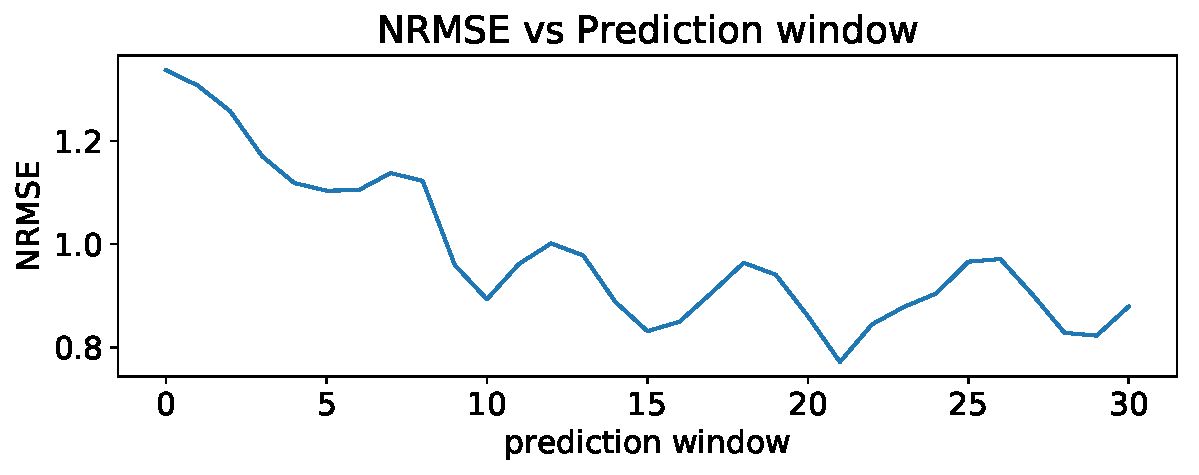
\includegraphics[width=\textwidth]{./results/images/nrmsevspwrec}

      \caption{NRMSE for different prediction window ranges}\label{fig:nrmsevspw}
  \end{figure}
 
 \begin{figure}[h]
    \centering
    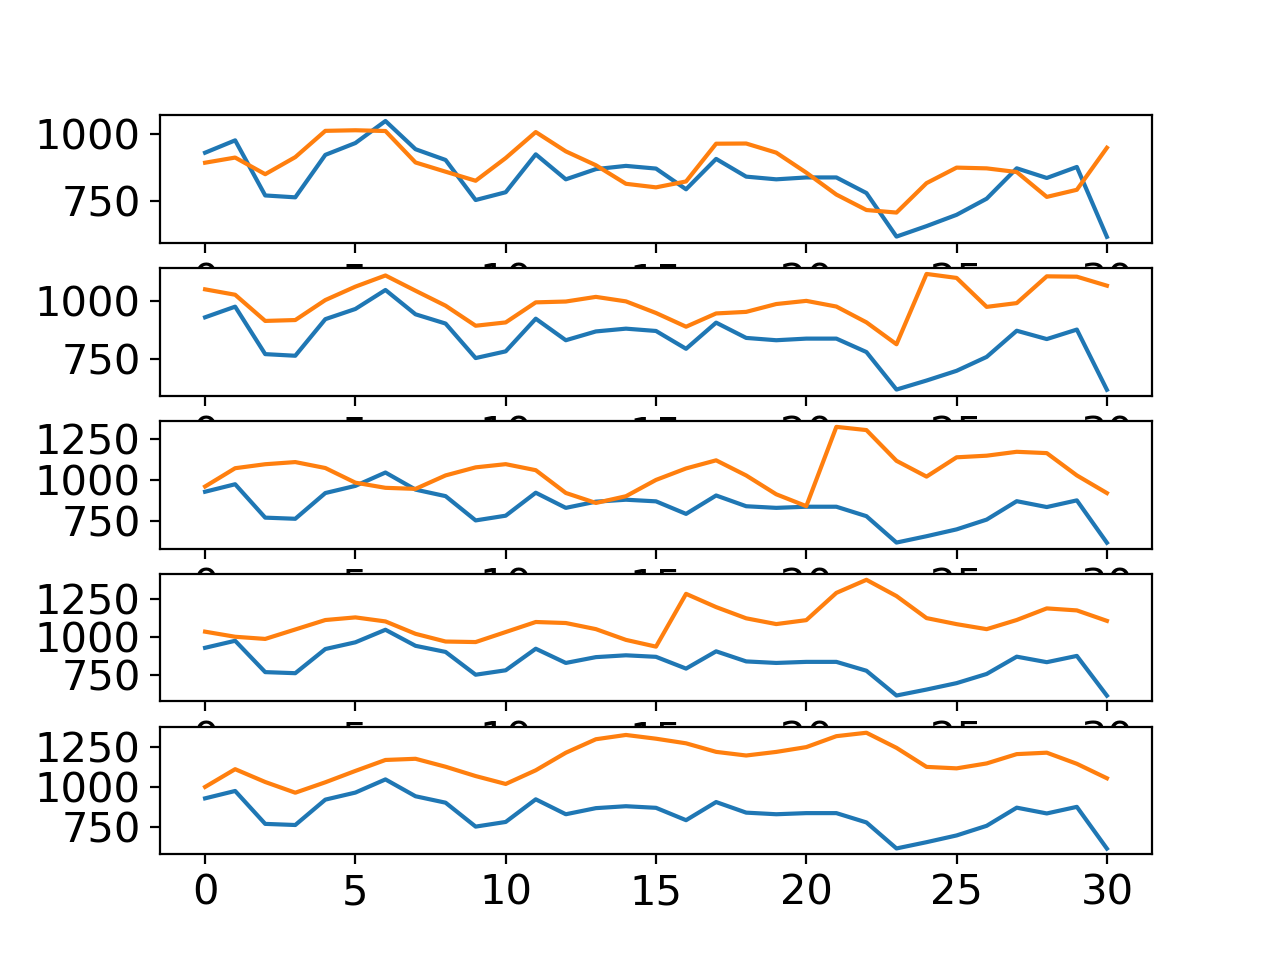
\includegraphics[width=\textwidth]{./results/images/realvspredicted}

     \caption{NRMSE for different prediction window ranges}\label{fig:realvspredicted}
 \end{figure}
 



  \section{Conclusions}

  Summarize the main aspects and results of the research
  project. Provide an answer to the research questions stated earlier.

  (target size: 1/2 page)

  \nocite{JS06}

  \newpage
  \bibliographystyle{unsrt}
  \bibliography{bibliography}

\end{document}

